\section{Introduction}

The integration of technology into the education system has accelerated, presenting nearly limitless opportunities for fostering cognitive development in children of all ages.

Technology has the potential to enhance various skills, including language proficiency, fine motor skills, memory, and attention, making it an invaluable tool in educational settings.

In light of this potential, this project proposes a solution aimed at the special education sector, specifically benefiting children with sensory and motor skill challenges, poor lateralization, and even older adults recovering from strokes.

The project employs a gyroscope sensor to detect inclination, calculate the state, and update the display, thereby illustrating key principles to children. Communication with the board is facilitated through the \textbf{I\textsuperscript{2}C} protocol.

To streamline the interaction between these components, predetermined libraries have been utilized.

To capture and maintain children's interest more effectively, an RGB palette has been chosen.

The primary goal is to enhance the therapy process in occupational therapy for children with special needs and to support their developmental progress.  \\

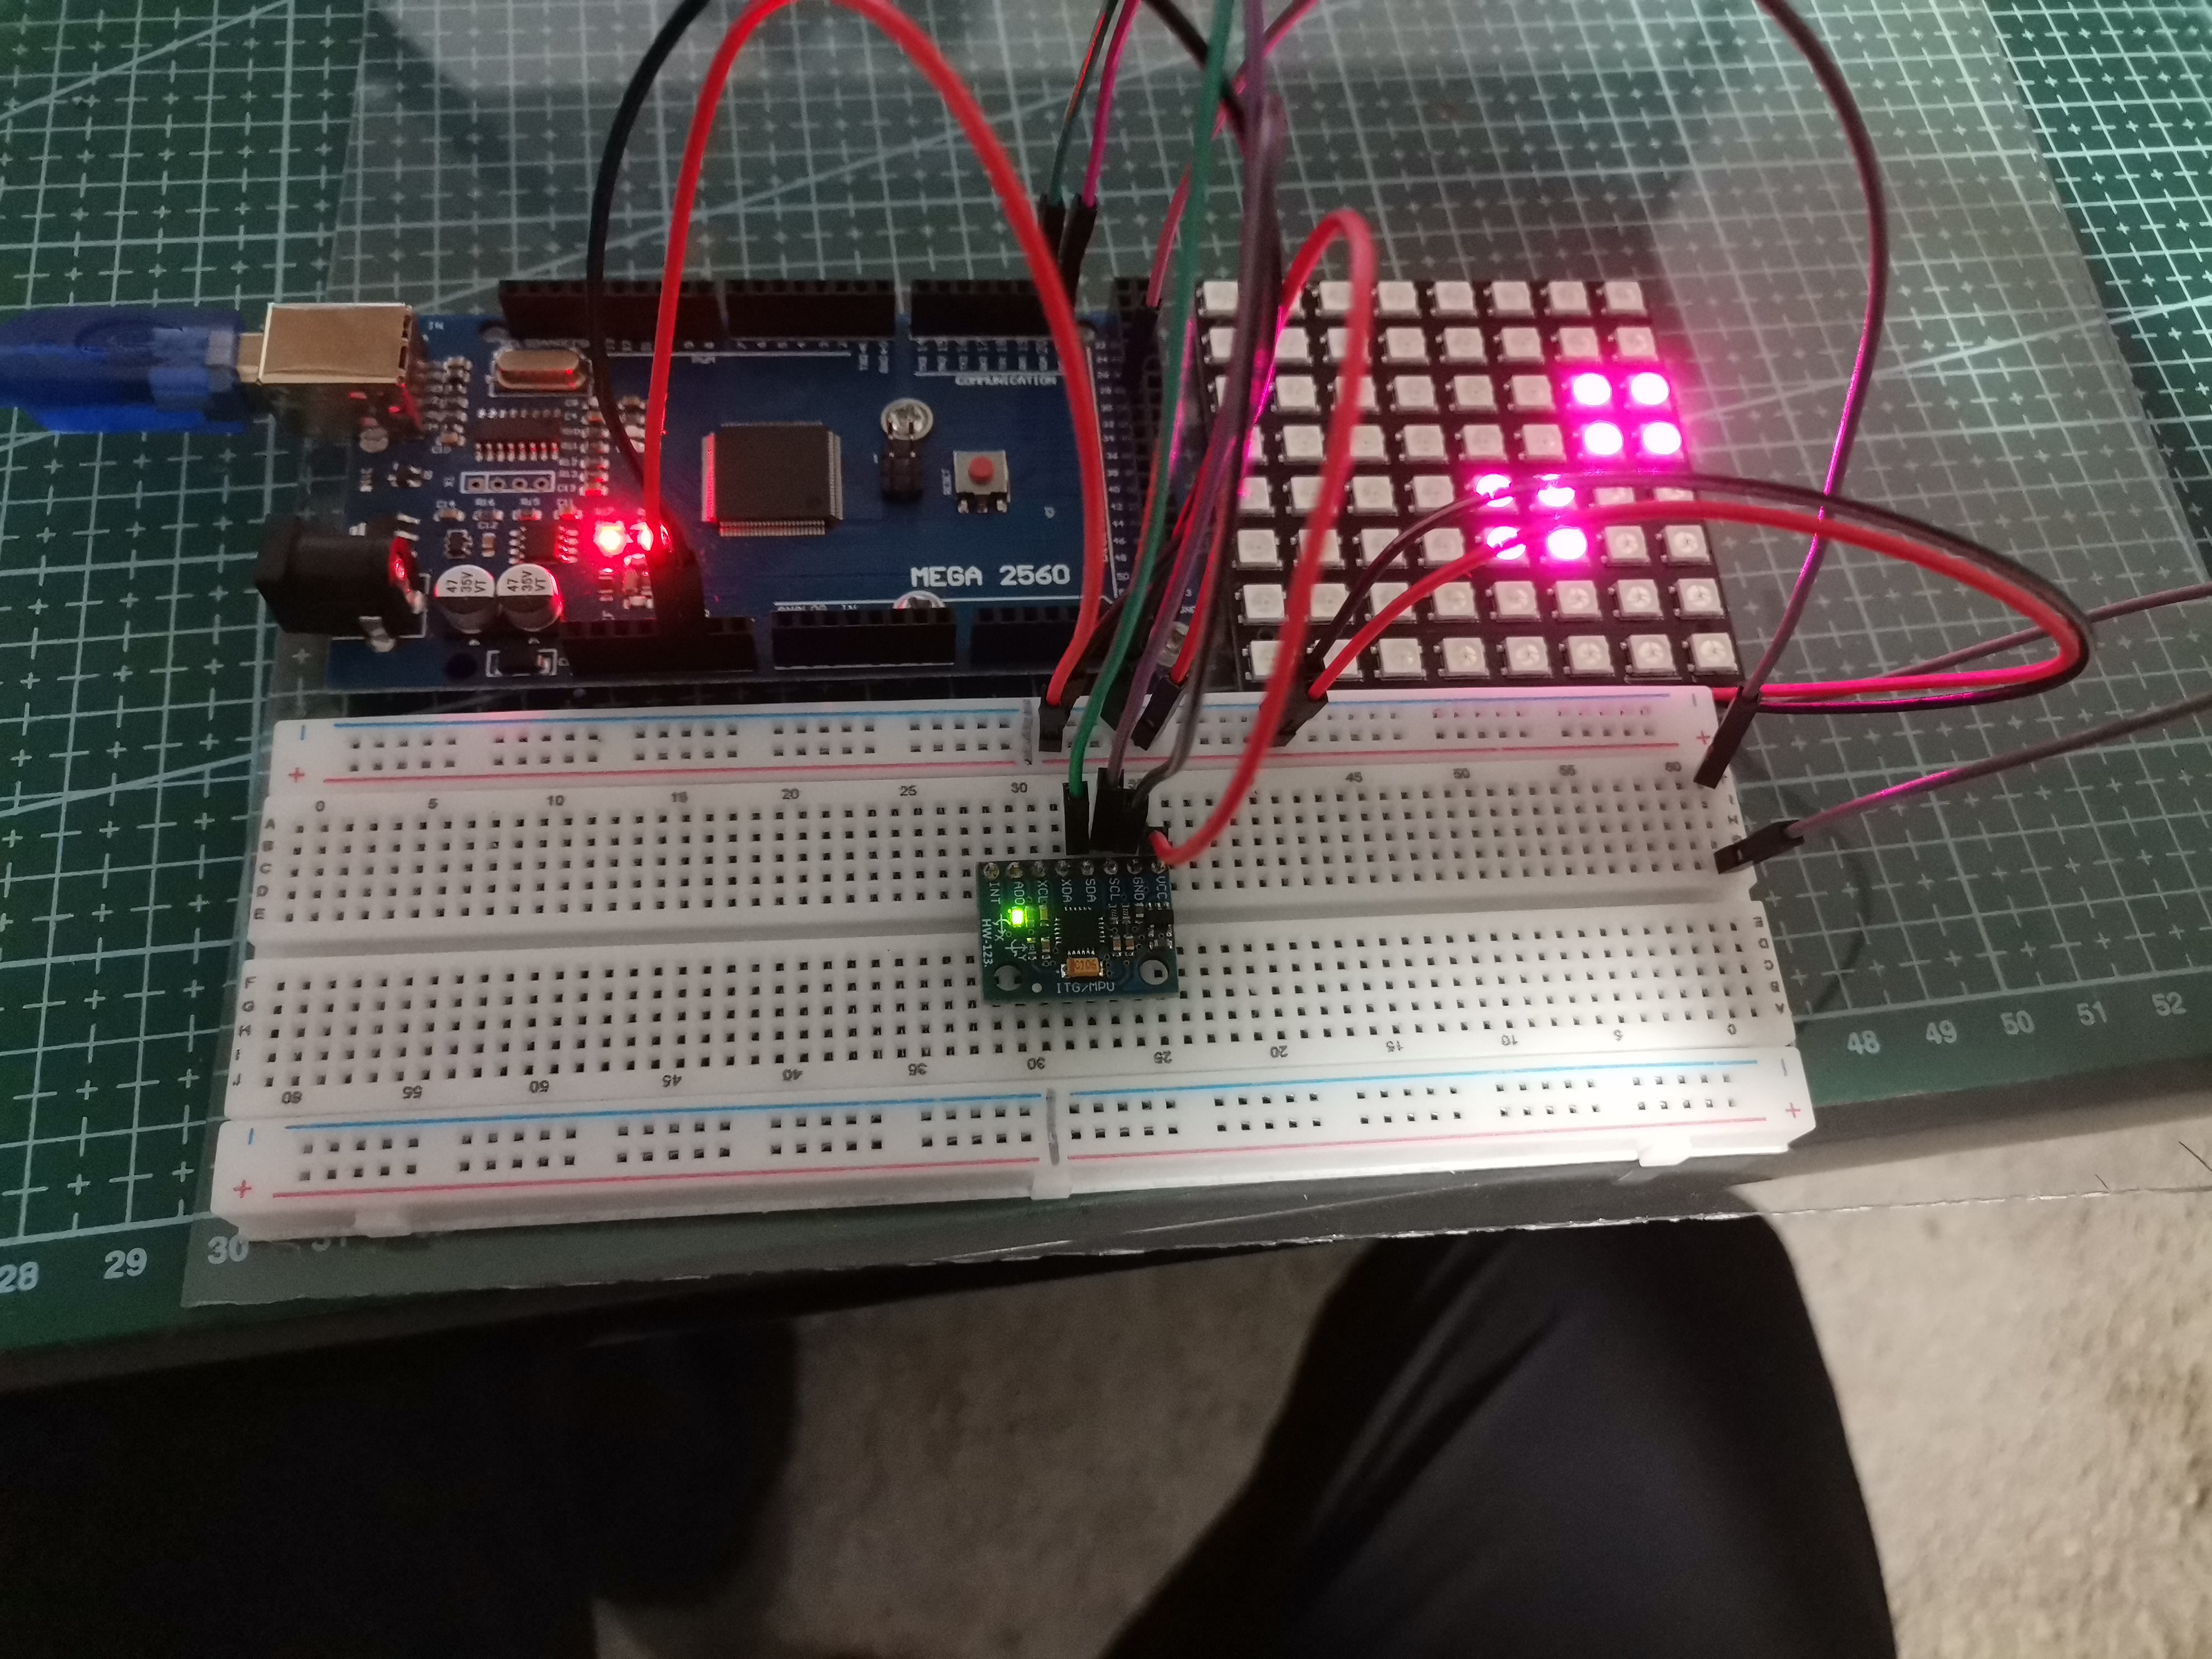
\includegraphics[width=1.0\linewidth]{demo/demo4.jpg}
